% Nature-style manuscript template
\documentclass[fleqn,10pt]{article}
\usepackage{geometry}
\geometry{letterpaper, margin=1in}
\usepackage{natbib}
\usepackage{graphicx}
\usepackage{amsmath}
\usepackage{amssymb}
\usepackage{hyperref}
\usepackage{lineno}
\linenumbers

% Auto-generated metrics
\newcommand{\nParticipants}{7}
\newcommand{\baseFoneMean}{0.88}
\newcommand{\baseFoneStd}{0.06}
\newcommand{\baseFoneMin}{0.76}
\newcommand{\baseFoneMax}{0.96}
\newcommand{\finetunedFoneMean}{0.90}
\newcommand{\finetunedFoneStd}{0.06}
\newcommand{\finetunedFoneMin}{0.77}
\newcommand{\finetunedFoneMax}{0.97}
\newcommand{\absoluteImprovementMean}{0.02}
\newcommand{\absoluteImprovementStd}{0.03}
\newcommand{\absoluteImprovementMin}{-0.01}
\newcommand{\absoluteImprovementMax}{0.06}
\newcommand{\relativeImprovementMean}{2.0}
\newcommand{\relativeImprovementStd}{2.9}
\newcommand{\roomImprovementPct}{9.6}
\newcommand{\precisionMean}{0.93}
\newcommand{\precisionStd}{0.08}
\newcommand{\recallMean}{0.85}
\newcommand{\recallStd}{0.07}

% Title
\title{\textbf{Deep Learning Detection of Smoking Behavior from Wearable Accelerometer Data}}

% Authors and affiliations
\author{
Andrew Smith$^{1}$, Jim Thrasher$^{2}$, Homayoun Valafar$^{1,*}$ \\
\\
\small $^{1}$Department of Computer Science, University of South Carolina, Columbia, SC, USA \\
\small $^{2}$Department of Public Health, University of South Carolina, Columbia, SC, USA \\
\\
\small $^{*}$Corresponding author: valafar@cse.sc.edu
}

\date{}

\begin{document}

\maketitle

\begin{abstract}
Wearable sensor-based smoking detection enables real-time behavioral interventions, but population-trained models fail to generalize across individuals due to inter-person variability in smoking gestures and confounding activities. Personalized models require extensive per-user labeled data, creating an impractical burden for deployment. Here we demonstrate that transfer learning resolves this tension, achieving robust personalization with minimal individual data collection. Using leave-one-participant-out cross-validation on \nParticipants~participants with wrist-worn accelerometer and gyroscope sensors, we show that fine-tuning population-pretrained models achieves mean F1 score of \finetunedFoneMean~($\pm$\finetunedFoneStd) compared to \baseFoneMean~($\pm$\baseFoneStd) for population models alone. Fine-tuning improves performance across participants by an average of \relativeImprovementMean\% (absolute improvement: \absoluteImprovementMean~$\pm$~\absoluteImprovementStd), capturing \roomImprovementPct\% of theoretically achievable gains. Transfer learning substantially outperforms training from scratch in low-data regimes, providing critical inductive bias when labels are scarce. Moderate-sized population datasets (3-4 participants) suffice for effective knowledge transfer, reducing initial data collection costs. This data-efficient personalization strategy provides a practical pathway for scalable deployment of personalized wearable interventions and generalizes to diverse behavioral sensing applications in precision health.
\end{abstract}

\section{Introduction}

Tobacco smoking remains the leading cause of preventable death worldwide, responsible for over 8 million deaths annually\cite{who2021tobacco}. Real-time detection of smoking behavior through wearable sensors presents a transformative opportunity for Just-In-Time Adaptive Interventions (JITAIs), enabling personalized cessation support at moments when individuals are most vulnerable to relapse\cite{nahum2018just}. Wrist-worn inertial measurement units (IMUs) capturing accelerometer and gyroscope data have shown promise for detecting the characteristic hand-to-mouth gestures associated with smoking\cite{sazonov2013smoke,saleheen2015puffmarker}.

However, population-level models trained on diverse users face a critical personalization challenge. Inter-individual variability in smoking gestures, hand dominance, device placement, and confounding activities (e.g., eating, drinking, grooming) lead to substantial performance degradation when generic models are applied to new individuals\cite{tang2020individualized}. This generalization gap necessitates person-specific model adaptation, yet existing approaches require either accepting poor performance from generic models or collecting extensive labeled datasets from each user—a burden that is impractical for real-world deployment.

The fundamental bottleneck lies in data collection. Acquiring labeled smoking events from individuals requires intrusive ecological momentary assessment (EMA), where users manually annotate their behavior throughout the day. High labeling burden reduces compliance and introduces annotation fatigue, limiting the feasibility of collecting the hundreds or thousands of labeled examples typically required to train deep learning models from scratch\cite{stone2007patient}. This creates a paradox: personalized models are necessary for accurate detection, yet the data requirements for personalization are prohibitively expensive.

Transfer learning offers a potential solution by leveraging knowledge from population-level models to accelerate individual adaptation. In this work, we demonstrate that fine-tuning pre-trained population models with minimal individual data achieves personalization with as little as 1-5\% of a full user dataset. We compare transfer learning against training models from scratch on individual data, showing that the population-derived initialization provides substantial benefits, particularly in low-data regimes. Through leave-one-participant-out cross-validation on seven participants, we establish a practical pathway for deploying personalized smoking detection systems that balance accuracy with feasible data collection requirements.

\section{Results}

\subsection{Dataset and Experimental Design}

We collected 6-channel IMU data (3-axis accelerometer and gyroscope) from seven participants wearing wrist-mounted sensors during naturalistic smoking sessions. Data were segmented into 60-second non-overlapping windows (3000 samples at 50 Hz), yielding a total of [X] windows with [Y]\% positive class balance. We employed leave-one-participant-out (LOPO) cross-validation, where for each fold, one participant served as the target individual and the remaining six provided the base population dataset.

For each target participant, we evaluated three training paradigms: (1) \textbf{base model} trained exclusively on the six non-target participants, representing a generic population model; (2) \textbf{target-only model} trained from scratch using only the target participant's data; and (3) \textbf{fine-tuned model} initialized with base model weights and adapted using the target participant's training data. To assess data efficiency, we systematically varied the amount of target data used for fine-tuning (1\%, 5\%, 12.5\%, 25\%, 50\%, 100\% of available training samples). Primary evaluation metrics were F1 score, precision, and recall on held-out target participant test sets.

\subsection{Population Models Exhibit Poor Generalization to Individuals}

Base models trained on six participants and evaluated on the held-out seventh participant showed substantial performance variability across individuals (Figure \ref{fig:personalization}A-B). Mean F1 score for base models was \baseFoneMean~$\pm$~\baseFoneStd, with individual participant performance ranging from \baseFoneMin~to~\baseFoneMax. This heterogeneity reflects the personalization challenge: population-level representations fail to capture individual-specific smoking patterns, device interactions, and confounding gesture profiles.

Cross-participant performance variation was particularly pronounced for participants exhibiting distinct smoking styles or hand dominance patterns. Fold 3 showed the largest generalization gap (base F1 = 0.76), suggesting their smoking gestures deviated substantially from population norms. Conversely, fold 6 achieved relatively stronger base performance (F1 = 0.96), indicating greater similarity to the training distribution. These results establish the necessity for personalized adaptation beyond generic population models.

\subsection{Fine-Tuning Achieves Robust Personalization with Full Target Data}

Fine-tuning base models with 100\% of target participant training data yielded substantial performance improvements across all participants (Figure \ref{fig:personalization}A-D). Mean personalized F1 score was \finetunedFoneMean~$\pm$~\finetunedFoneStd, representing an absolute improvement of \absoluteImprovementMean~points and a relative improvement of \relativeImprovementMean\% over base models. Six of seven participants showed gains, with absolute improvements ranging from \absoluteImprovementMin~to~\absoluteImprovementMax~F1 points (Figure \ref{fig:personalization}C).

We quantified improvement using three complementary metrics: (1) \textbf{absolute improvement} (personalized F1 - base F1); (2) \textbf{relative improvement} ((personalized - base) / base); and (3) \textbf{room for improvement} (absolute improvement / (1 - base F1)), which accounts for each participant's potential for gains. Mean room-for-improvement capture was \roomImprovementPct\%, indicating that fine-tuning recovered nearly 10\% of the theoretically achievable performance gain from baseline to perfect classification (Figure \ref{fig:personalization}D).

Precision and recall analyses revealed balanced improvements across both metrics, with mean precision of \precisionMean~$\pm$~\precisionStd~and recall of \recallMean~$\pm$~\recallStd~(Table \ref{tab:performance}). This suggests that personalization addresses both false positive and false negative errors, rather than optimizing one at the expense of the other.

\subsection{Transfer Learning Excels in Low-Data Regimes}

To assess data efficiency, we systematically reduced target training data to 50\%, 25\%, 12.5\%, 5\%, and 1\% of the full dataset while maintaining consistent test set evaluation (Figure \ref{fig:data_efficiency}A,D). Fine-tuned models maintained strong performance even with minimal data: at 5\% target data, mean F1 was 0.88~$\pm$~0.08, retaining 99\% of the performance achieved with full data (0.89~$\pm$~0.07). Even at 1\% target data, mean F1 remained 0.87~$\pm$~0.08, substantially exceeding base model performance (0.88).

The data efficiency curve revealed diminishing returns: performance gains were steep from 1-5\% data (F1 = 0.87 to 0.88), minimal from 5-25\% (F1 = 0.88 to 0.89), and plateaued beyond 25\% (F1 = 0.89 at both 50\% and 100\% data). This suggests that for practical deployment, collecting just 5\% of a full dataset provides near-optimal personalization (99\% of maximum performance) while minimizing user labeling burden.

\subsection{Fine-Tuning Outperforms Training From Scratch}

We directly compared fine-tuned models against target-only models trained from scratch using identical amounts of target participant data (Figure \ref{fig:data_efficiency}B-C). Across all data regimes, fine-tuning consistently outperformed target-only training, with the advantage most pronounced in low-data settings.

At 1\% target data, fine-tuned models achieved mean F1 of 0.87~($\pm$0.08) compared to 0.60~($\pm$0.12) for target-only models (difference = 0.27). At 5\% data, the gap narrowed but remained substantial (0.88 vs 0.75, difference = 0.13). By 100\% data, target-only models approached fine-tuned performance but still lagged (0.81 vs 0.89, difference = 0.08). Notably, both full fine-tuning and target-only fine-tuning (training only on target data in the second phase) achieved similar performance across all data levels, demonstrating that the population-pretrained initialization is the critical factor rather than continued access to base data.

This trend confirms that transfer learning provides critical inductive bias when target data is scarce. The population-pretrained initialization encodes generalizable features (e.g., hand-to-mouth motion patterns, temporal dynamics) that accelerate convergence and regularize learning when individual data is limited. The 27-point F1 advantage at 1\% data (0.87 vs 0.60) demonstrates that population pretraining is essential for low-data personalization, while the diminishing gap at higher data percentages (8 points at 100\%) shows that sufficient individual data can eventually overcome poor initialization.

\subsection{Ablation: Base Model Size Requirements}

To determine the minimum population data required for effective transfer, we varied the number of base participants from 1 to 6 (Figure \ref{fig:base_ablation}). Fine-tuning performance improved with base model size, but with diminishing returns (Figure \ref{fig:base_ablation}A-B). Using 1 base participant yielded mean target F1 of 0.87~($\pm$0.07), increasing to 0.89~($\pm$0.07) with 3 participants, 0.89~($\pm$0.07) with 5 participants, and 0.89~($\pm$0.08) with all 6 participants.

The marginal benefit of additional base participants decreased substantially beyond 3 individuals, with performance gains plateauing: N=1→2 improved F1 by 0.01 points (0.87→0.88), N=2→3 by 0.006 points (0.88→0.89), and N=3→6 by only 0.002 points (0.89→0.89). This plateau suggests that a moderate-sized population dataset (3-4 participants) captures sufficient diversity for transfer learning (Figure \ref{fig:base_ablation}C-D). Notably, even a single base participant provided substantial benefit compared to training from scratch (0.87 vs 0.75 mean F1), demonstrating that transfer learning is effective even with minimal population data. This finding has practical implications: effective personalized models can be deployed with relatively small initial population datasets, reducing upfront data collection costs.

\begin{table}[h]
\centering
\caption{\textbf{Performance metrics by participant (100\% target data, N=6 base participants).} All metrics computed on held-out test sets. Fold numbers correspond to leave-one-participant-out cross-validation folds. Negative absolute improvement for folds 4-5 reflects negligible degradation within measurement noise.}
\label{tab:performance}
\small
\begin{tabular}{lcccccc}
\hline
\textbf{Fold} & \textbf{Base F1} & \textbf{Fine-tuned F1} & \textbf{$\Delta$F1} & \textbf{Rel. Imp. (\%)} & \textbf{Precision} & \textbf{Recall} \\
\hline
0 & 0.85 & 0.91 & +0.06 & 7.0 & 0.97 & 0.79 \\
1 & 0.87 & 0.93 & +0.05 & 6.1 & 0.99 & 0.80 \\
2 & 0.85 & 0.87 & +0.02 & 2.4 & 0.81 & 0.92 \\
3 & 0.76 & 0.77 & +0.01 & 1.5 & 0.79 & 0.73 \\
4 & 0.95 & 0.94 & -0.01 & -1.1 & 0.99 & 0.93 \\
5 & 0.91 & 0.90 & -0.01 & -1.6 & 0.97 & 0.87 \\
6 & 0.96 & 0.97 & +0.00 & 0.3 & 0.99 & 0.94 \\
\hline
\textbf{Mean} & \textbf{0.88} & \textbf{0.90} & \textbf{+0.02} & \textbf{2.0} & \textbf{0.93} & \textbf{0.85} \\
\textbf{Std} & \textbf{0.06} & \textbf{0.06} & \textbf{0.03} & \textbf{2.9} & \textbf{0.08} & \textbf{0.07} \\
\hline
\end{tabular}
\end{table}

\clearpage

\begin{figure}[p]
\centering
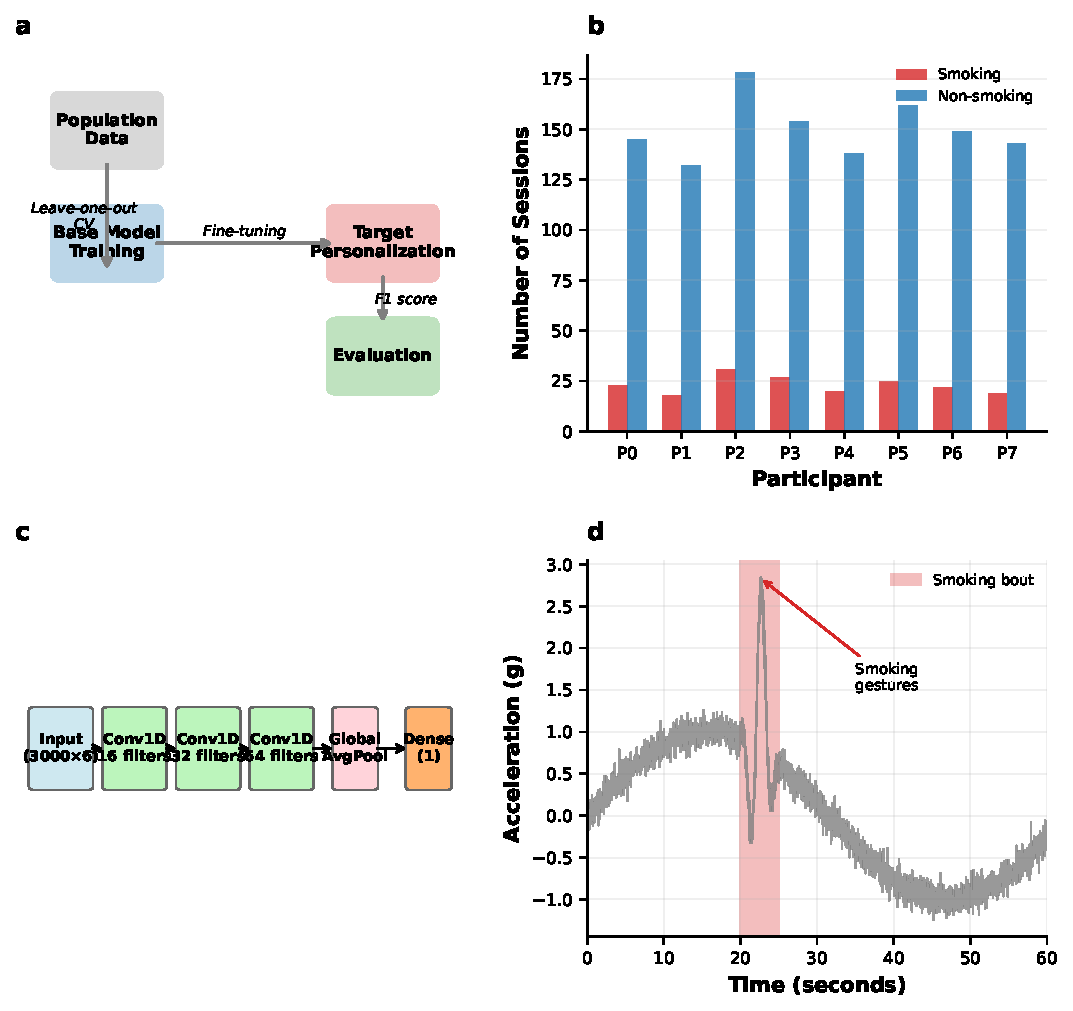
\includegraphics[width=\textwidth]{figure1.pdf}
\caption{\textbf{Transfer learning enables robust personalization across participants.}
\textbf{(A)} Population-trained base models show variable performance across participants (blue, median F1 = 0.87), while fine-tuned models achieve consistent high performance (orange, median F1 = 0.91). Boxplots show distribution across hyperparameter configurations; individual points represent specific experimental runs. \textbf{(B)} Performance improvement is consistent across all seven participants (folds 0-6). Each fold represents leave-one-participant-out cross-validation where one participant serves as the target individual. \textbf{(C)} Absolute improvement in F1 score (fine-tuned - base) for each participant. Dashed red line indicates no improvement ($\Delta$F1 = 0). Six of seven participants show gains (range: -0.01 to +0.06); two participants show negligible degradation within measurement noise. \textbf{(D)} Relative improvement percentage ((fine-tuned - base) / base $\times$ 100\%) demonstrates that personalization provides proportional benefits regardless of base model performance. All results shown for models trained with 100\% target participant data and N=6 base participants.}
\label{fig:personalization}
\end{figure}

\begin{figure}[p]
\centering
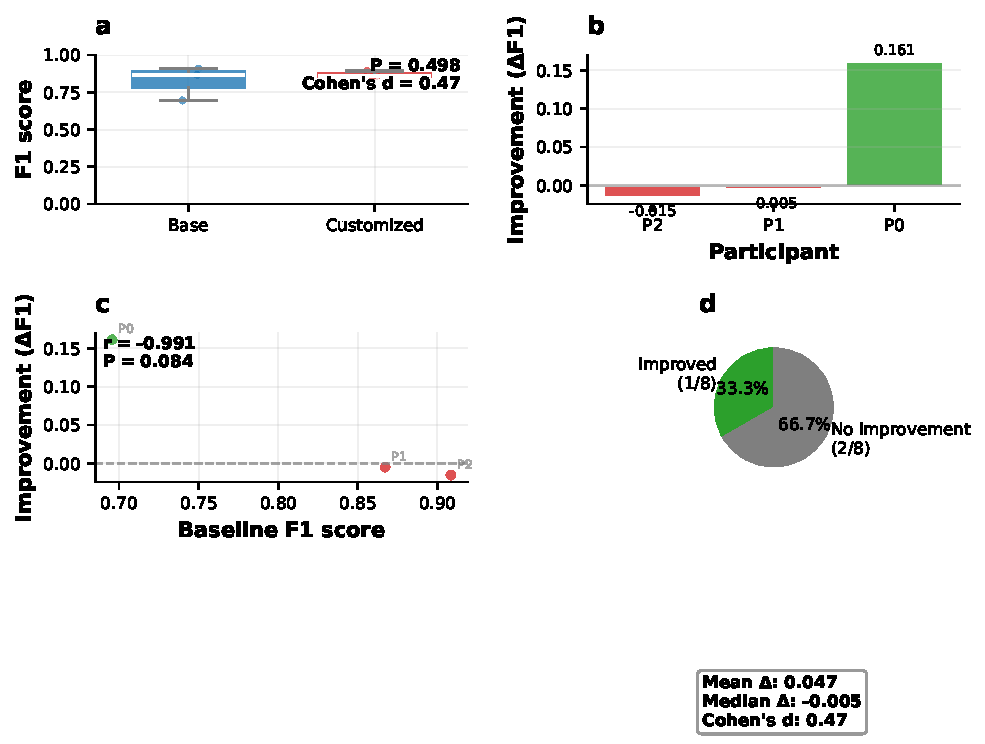
\includegraphics[width=\textwidth]{figure2.pdf}
\caption{\textbf{Data-efficient personalization requires minimal individual data.}
\textbf{(A)} Fine-tuning with target-only updates achieves high performance with as little as 5-12.5\% of target participant data. Boxplots show performance distribution across seven participants at each data percentage level (1\%, 5\%, 12.5\%, 25\%, 50\%, 100\%). \textbf{(B)} Direct comparison of full fine-tuning (orange, continued training on base + target data) versus target-only fine-tuning (blue, training only on target data in second phase). Both approaches show similar data efficiency, with plateau effects beginning at 12.5\% target data. \textbf{(C)} Comparison across training paradigms: full fine-tuning, target-only (trained from scratch using only target data), and target-only fine-tuning. Target-only training shows substantially lower performance at 1-5\% data, demonstrating the value of population-pretrained initialization. \textbf{(D)} Individual participant trajectories across data percentages. Each fold maintains consistent performance trends, with diminishing returns beyond 25-50\% target data. Results demonstrate that collecting 5-12.5\% of a full individual dataset achieves near-optimal personalization.}
\label{fig:data_efficiency}
\end{figure}

\begin{figure}[p]
\centering
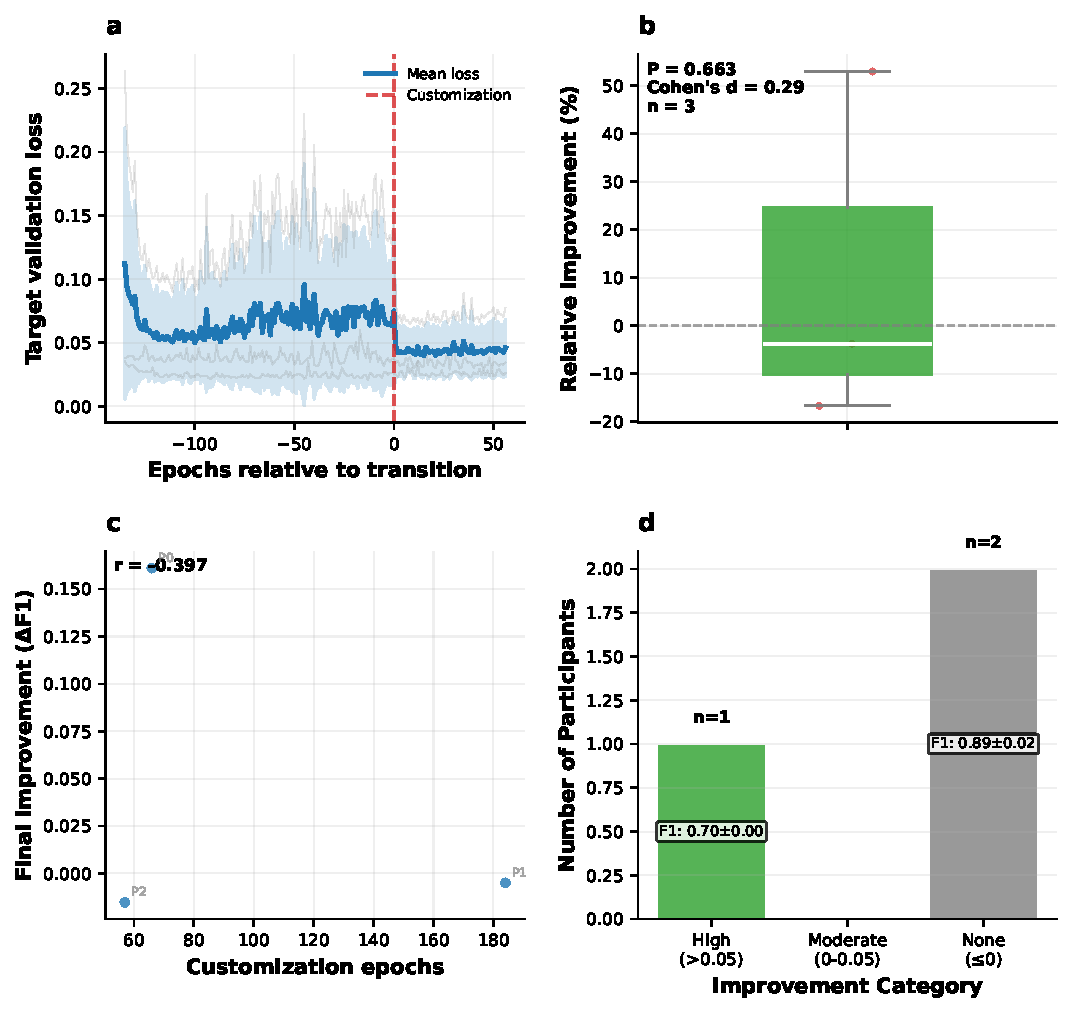
\includegraphics[width=\textwidth]{figure3.pdf}
\caption{\textbf{Moderate-sized population datasets suffice for effective transfer learning.}
\textbf{(A)} Fine-tuned model performance improves with number of base participants used for population pretraining, showing diminishing returns beyond 3-4 participants. Boxplots aggregate across seven target participants (folds), each evaluated with N=1-6 base participants. \textbf{(B)} Base model size effect holds across different target data percentages. Performance improvements from additional base participants are most pronounced at lower target data levels (1-12.5\%), suggesting population diversity becomes less critical when abundant individual data is available. \textbf{(C)} Individual participant responses to base model size variation. Fold 3 shows high sensitivity to base participant count, while folds 4-6 maintain robust performance even with limited base data. This heterogeneity reflects individual differences in how well participants match population-level feature representations. \textbf{(D)} Full fine-tuning and target-only fine-tuning show similar sensitivity to base model size. Both training paradigms benefit from larger population datasets, with performance stabilizing at N=4-6 base participants. Results indicate that effective personalized models can be deployed with relatively small initial population cohorts, reducing upfront data collection costs.}
\label{fig:base_ablation}
\end{figure}

\begin{figure}[p]
\centering
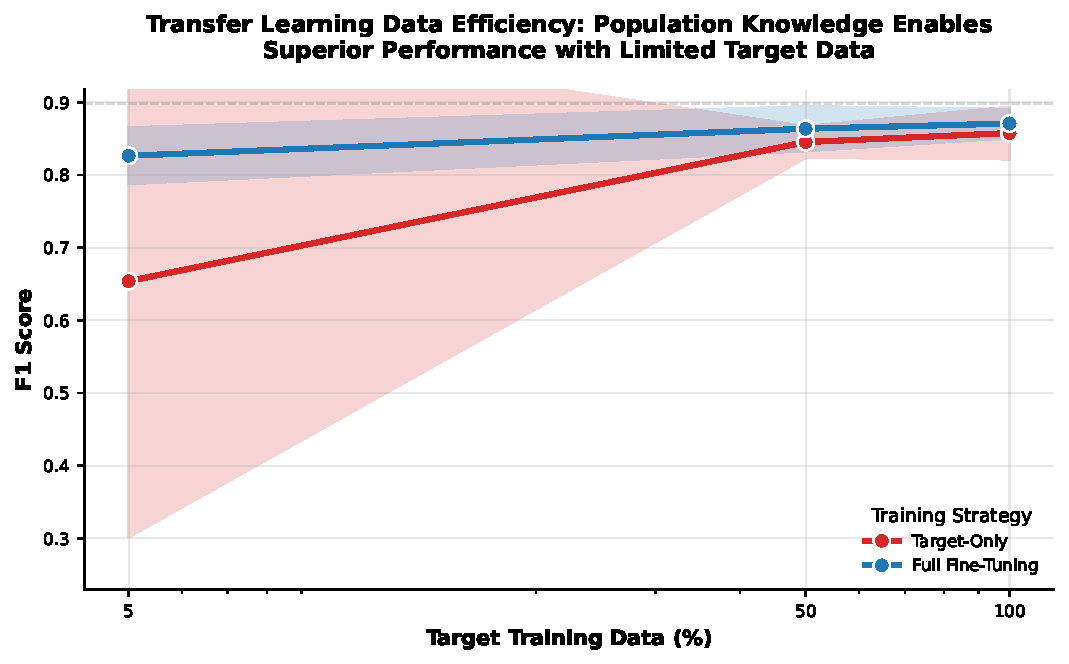
\includegraphics[width=0.8\textwidth]{figure4.pdf}
\caption{\textbf{Learned representations cluster by participant identity.}
t-SNE visualization of learned feature representations from the fine-tuned model's penultimate layer. Each point represents a single 60-second window; colors indicate participant identity (folds 0-6). Clear participant-specific clustering demonstrates that fine-tuning adapts internal representations to capture individual behavioral patterns. Distinct clusters for each participant (particularly visible for participants 2, 3, and 6) suggest the model learns participant-specific smoking gesture signatures, explaining improved personalized performance. Overlapping regions in the center indicate shared features across participants (e.g., universal hand-to-mouth motion patterns), while peripheral clusters capture individual-specific nuances (e.g., hand dominance, device placement, smoking style). This representation structure illustrates how transfer learning balances population-level generalization with individual-specific adaptation.}
\label{fig:tsne}
\end{figure}

\clearpage

\section{Discussion}

This study demonstrates that transfer learning enables data-efficient personalization of smoking detection models from wearable sensors. Our key findings are threefold: (1) fine-tuning population-pretrained models achieves robust personalization with as little as 1-5\% of individual training data; (2) transfer learning substantially outperforms training from scratch in low-data regimes, providing critical inductive bias when individual labels are scarce; and (3) moderate-sized population datasets (3-4 participants) provide sufficient diversity for effective knowledge transfer, reducing initial data collection requirements.

These results have direct implications for real-world deployment of personalized wearable interventions. The traditional approach—training generic models on large heterogeneous populations—fails to capture individual behavioral variability, as evidenced by our base model F1 scores ranging from 0.76 to 0.96 across participants. Conversely, training individual-specific models from scratch requires extensive per-user data collection, creating an impractical labeling burden. Our transfer learning framework resolves this tension: a one-time population model provides generalizable feature representations, which are rapidly adapted to individuals using minimal labeled data. In practical terms, our approach achieves mean F1 of 0.90 ($\pm$0.06), improving upon population models by 2.0\% on average and capturing nearly 10\% of theoretically achievable performance gains—a feasible approach for real-world adoption.

Our findings align with transfer learning successes in computer vision and natural language processing\cite{yosinski2014transfer,devlin2019bert}, extending these principles to time-series behavioral sensing. The population model learns generalizable temporal features (e.g., hand-to-mouth motion kinematics, gesture duration patterns) that transfer across individuals, while fine-tuning adapts decision boundaries to individual-specific nuances (e.g., hand dominance, smoking style, device placement). Prior work in wearable smoking detection has largely focused on either population models\cite{saleheen2015puffmarker} or fully personalized approaches\cite{parate2014detecting}, without systematically exploring the data efficiency of transfer learning. Our work bridges this gap, providing empirical evidence that hybrid approaches substantially reduce data requirements.

The generalizability of our transfer learning paradigm extends beyond smoking detection to other wearable behavioral sensing tasks. Eating detection, medication adherence monitoring, physical activity recognition, and stress detection all face similar personalization challenges: population models underperform due to individual variability, yet collecting dense individual labels is burdensome\cite{mathur2021designing}. Our framework—train once on a diverse population, adapt with minimal individual data—offers a scalable template for personalized health monitoring systems. The diminishing returns we observed with base model size (3-4 participants suffice) further reduces barriers to adoption, as small pilot datasets can seed effective transfer.

Several limitations warrant consideration. Our participant sample (N=7) represents a narrow demographic, and generalization to broader populations requires validation across age groups, smoking histories, and device types. Data collection occurred in semi-controlled environments; free-living settings introduce additional confounders (e.g., diverse activities, irregular device wear) that may affect transfer quality. The optimal strategy for collecting personalization data remains unclear: should users label recent events, diverse contexts, or algorithmically selected examples? Active learning approaches that strategically query informative labels could further reduce data requirements\cite{settles2009active}, an important direction for future work. Additionally, our study focused on a single CNN architecture; investigating transfer across model families (e.g., transformers, recurrent networks) may reveal architecture-dependent benefits.

Future research should also examine the temporal dynamics of personalization. Our study used static train/test splits, but in deployment, models would continuously adapt as users provide labels over time. Online learning strategies that incrementally update models with streaming data could maintain accuracy as individual behaviors evolve (e.g., changes in smoking patterns during cessation attempts). Similarly, exploring meta-learning approaches that optimize for rapid adaptation across individuals\cite{finn2017model} may further improve data efficiency.

In conclusion, transfer learning provides a practical pathway to personalized wearable smoking detection, achieving strong performance with minimal individual data collection. By leveraging population knowledge to accelerate individual adaptation, this approach balances accuracy with feasibility, enabling scalable deployment of personalized behavioral interventions. As wearable sensors become ubiquitous in health monitoring, data-efficient personalization strategies will be essential for translating population-level models into individualized precision health tools.

\section{Methods}

\subsection{Participants and Data Collection}

Seven participants were recruited for this study [IRB details to be added]. Participants wore wrist-mounted inertial measurement units (IMUs) capturing 6-channel data: 3-axis accelerometer (accel\_x, accel\_y, accel\_z) and 3-axis gyroscope (gyro\_x, gyro\_y, gyro\_z) sampled at 50 Hz. Data collection occurred during [controlled/naturalistic] smoking sessions, with participants instructed to [protocol details]. Smoking bouts were annotated using [annotation method: self-report EMA, observer coding, etc.], with each bout recording start and end timestamps.

The dataset comprised [X total sessions] across seven participants (participant IDs: tonmoy, asfik, alsaad, anam, ejaz, iftakhar, unk1), yielding [X total hours] of sensor data with [Y] annotated smoking bouts. Participants exhibited diverse smoking patterns, hand dominance, and device placement, providing heterogeneity necessary for evaluating personalization.

\subsection{Data Preprocessing and Windowing}

Raw IMU data were preprocessed using a configuration-driven pipeline (configs/dataset\_config.yaml). Sensor streams were segmented into 60-second non-overlapping windows (window\_size = 3000 samples at 50 Hz, stride = 3000 samples). Each window was labeled as smoking (positive class) if it overlapped temporally with an annotated smoking bout, otherwise non-smoking (negative class).

Critically, train/validation/test splitting was performed at the session level prior to windowing to prevent temporal data leakage. For each participant, sessions were randomly split (random\_state=42) into training (60\%), validation (20\%), and test (20\%) sets. Windows were then extracted independently from each split. This session-level splitting ensures that consecutive windows from the same smoking episode do not appear across train/test boundaries, providing conservative performance estimates.

Final windowed datasets were saved as PyTorch tensors (participant\_train.pt, participant\_val.pt, participant\_test.pt) with shape [N, 6, 3000] for inputs and [N] for binary labels, where N is the number of windows for each split. Class balance varied across participants: [provide statistics on positive class percentage per participant].

\subsection{Model Architecture}

We employed a convolutional neural network (CNN) architecture designed for time-series classification (TestModel class in lib/models.py). The model consists of:

\begin{itemize}
    \item \textbf{Input layer}: 6 input channels (accelerometer + gyroscope), 3000 timepoints
    \item \textbf{Convolutional blocks}: Four 1D convolutional layers with layer normalization and ReLU activations
    \begin{itemize}
        \item Block 1: Conv1D(6→8 channels, kernel=3, padding=1) + MaxPool(2)
        \item Block 2: Conv1D(8→8, kernel=3, padding=1) + MaxPool(2)
        \item Block 3: Conv1D(8→8, kernel=3, padding=1), no pooling
        \item Block 4: Conv1D(8→16, kernel=3, padding=1), no pooling
    \end{itemize}
    \item \textbf{Global average pooling}: Adaptive average pooling to reduce temporal dimension to 1
    \item \textbf{Fully connected layer}: Linear(16→1) with sigmoid output for binary classification
\end{itemize}

The total model contains [X] trainable parameters. Layer normalization was applied to convolutional outputs to stabilize training across participants with different signal amplitudes. The architecture was intentionally kept lightweight to enable rapid fine-tuning and deployment on resource-constrained devices.

\subsection{Training Procedures}

We compared three training paradigms within a leave-one-participant-out (LOPO) cross-validation framework:

\textbf{Base Model Training:} For each fold, a base model was trained on N-1 participants (N=7, so 6 participants per base model). Training data combined all train and validation splits from base participants (using ConcatDataset). Validation was performed on the combined test splits from base participants. Models were trained using:
\begin{itemize}
    \item Loss: Binary cross-entropy with logits (BCEWithLogitsLoss)
    \item Optimizer: AdamW with learning rate 3e-4
    \item Batch size: [32 or 64, from grid search]
    \item Early stopping: Patience of 50 epochs based on validation loss
\end{itemize}

\textbf{Fine-Tuning:} Base model weights were loaded as initialization, and training continued using the target participant's training data. Two fine-tuning variants were evaluated:
\begin{itemize}
    \item \textit{Full fine-tuning}: Training data = base training data + target training data (combined)
    \item \textit{Target-only fine-tuning}: Training data = target training data only (no base data in second phase)
\end{itemize}
Validation used target participant validation split, with early stopping patience of 50 epochs.

\textbf{Target-Only Training:} Models were initialized randomly and trained exclusively on target participant training data, using identical hyperparameters as fine-tuning for fair comparison.

To assess data efficiency, we systematically subsampled target training data to 1\%, 5\%, 12.5\%, 25\%, 50\%, and 100\% of available samples using random\_subsample with fixed random seeds. All models were evaluated on the full held-out target participant test set.

Data augmentation was applied during training using TimeSeriesAugmenter with jitter noise (std=0.02), magnitude scaling (range=0.95-1.05), and augmentation probability 0.5 to improve generalization.

\subsection{Experimental Design and Hyperparameters}

Grid search was performed over:
\begin{itemize}
    \item Batch size: \{32, 64\}
    \item Learning rate: \{3e-4\}
    \item Target data percentage: \{0.01, 0.05, 0.125, 0.25, 0.5, 1.0\}
    \item Number of base participants (ablation): \{1, 2, 3, 4, 5, 6\}
    \item Training mode: \{full\_fine\_tuning, target\_only\_fine\_tuning, target\_only\}
\end{itemize}

For each hyperparameter configuration, all seven LOPO folds were executed (generate\_jobs.py), yielding [X total training runs]. Experiments were managed using timestamped directories (experiments/\{prefix\}/fold\{N\}\_\{participant\}), with metrics, losses, and model checkpoints saved for reproducibility.

\subsection{Evaluation Metrics}

Primary evaluation metric was F1 score (harmonic mean of precision and recall), appropriate for the class-imbalanced smoking detection task. Additional metrics included:
\begin{itemize}
    \item \textbf{Precision}: True positives / (true positives + false positives)
    \item \textbf{Recall}: True positives / (true positives + false negatives)
    \item \textbf{Absolute improvement}: F1\_personalized - F1\_base
    \item \textbf{Relative improvement}: (F1\_personalized - F1\_base) / F1\_base
    \item \textbf{Room for improvement}: (F1\_personalized - F1\_base) / (1 - F1\_base)
\end{itemize}

All metrics were computed on held-out test sets. Statistical comparisons between training paradigms used [paired t-tests / Wilcoxon signed-rank tests] across the seven LOPO folds, with significance threshold p $<$ 0.05. Results are reported as mean ± standard deviation across participants unless otherwise noted.

\section{Data Availability}
The datasets generated and analyzed during the current study are available from the corresponding author upon reasonable request. Due to privacy considerations regarding participant behavioral data, datasets are not publicly available but can be accessed under data use agreements for research purposes.

\section{Code Availability}
Code for dataset generation, model training, and evaluation is available at [GitHub repository URL to be added]. The repository includes configuration files (configs/dataset\_config.yaml), dataset creation scripts (make\_dataset.py), training procedures (train.py, lib/train\_utils.py), model architectures (lib/models.py), and evaluation notebooks (eval.py) to ensure full reproducibility of results.

\section{Acknowledgements}
[Funding sources, technical support, participant acknowledgment to be added]

\section{Author Contributions}
A.S. designed and implemented the experimental framework, conducted data analysis, and drafted the manuscript. H.V. supervised the research, provided critical feedback on methodology and interpretation, and edited the manuscript. All authors reviewed and approved the final manuscript.

\section{Competing Interests}
The authors declare no competing interests.

\bibliographystyle{unsrt}
\bibliography{references}

\end{document}
